\chapter{Servidor de mapas dinámico}
\label{cap:sevidordemapasdinamico}


En este capítulo se explica la construcción y el funcionamiento del servidor de mapas dinámico. En primer lugar se explica que és, para que se utiliza y como se construye un \textit{costmap}. En segundo lugar se explica como se construyen los mapas que componen el algoritmo y por último se explica como se combinan estos mapas para generar el mapa usado en la navegación.

\section{Costmap\_2D}
\label{sec:costmap2d}
Un \textit{costmap} es una estructura de datos ofrecida por ROS y compuesta por un grid de ocupación y los metadatos de este grid. Cada celda del grid toma valores entre 0 y 255, donde 0 corresponde a una celda vacía, los valores entre 1 y 254 representan la probabilidad de que una celda está ocupada y el valor 255 se reserva para el desconocimiento. Cada valor se asocia con un nivel de gris, como se puede ver en la imagen.
\begin{figure} [hbtp]
  \begin{center}
    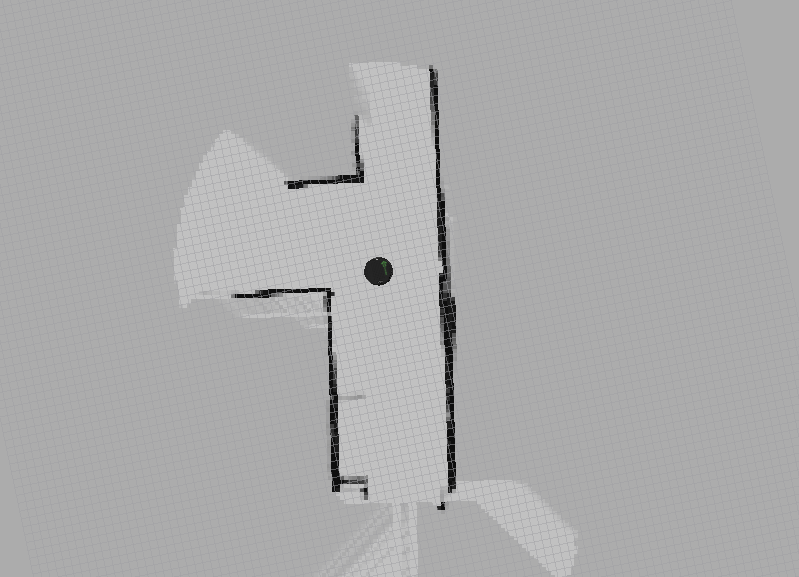
\includegraphics[width=7.5cm]{img/cap4/costmap-ejemplo}
  \end{center}
  \caption{Ejemplo visual de un costmap.}
  \label{fig:costmap-ejemplo}
\end{figure}\

Para poder representar la ocupación de un objeto en un \textit{costmap} es necesario hacer uso de las transformadas entre frames que nos ofrece ROS.

\subsubsection{tf}
\label{subsubsec:tf}
Cualquier robot está compuesto por multitud de piezas moviles, como puede ser la propia base del robot o la pinza de un brazo robótico. Cada una de estas piezas se pueden representar con un \textit{frame}. Ademas existen tambien otros \textit{frames} que pueden interesarnos, como puede ser el \textit{frame} de world o el \textit{frame} de map.
\begin{figure} [hbtp]
  \begin{center}
    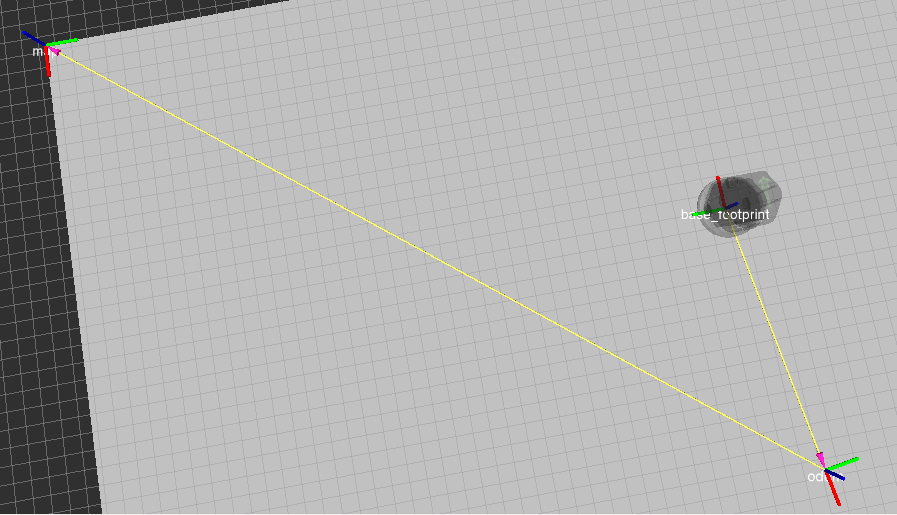
\includegraphics[width=12cm]{img/cap4/frames}
  \end{center}
  \caption{A la izquierda el frame map y a la derecha los frames de odom y base\_footprint}
  \label{fig:frames}
\end{figure}

Usamos las \textit{tf} para poder representar información relativa a uno de estos frames. Esto puede sernos de utilidad, por ejemplo, si queremos conocer la posición de un objeto que hemos cogido con nuestra pinza respecto a la base de nuestro robot, o cual es la posición relativa de un objeto que estamos percibiendo con el laser respecto a nosotros o respecto al mapa.

Cuando trabajamos con mapas es importante que todo lo que se representa en él sea respecto al frame map. De este modo nuestro mapa puede ser usado por otros nodos, como el nodo de navegación, o en cualquier otro escenario. \pagebreak

\section{Tipos de mapas}

En este apartado se describirá la metodologia seguida para la construcción de cada uno de los tres mapas usados por el algoritmo.

\subsection{Mapa estático}
El mapa estático se caracteriza por incluir las partes inmutables del escenario, como son las paredes o las puertas. La mejor manera de construirlo es medir todo el escenario y crear el mapa usando una herramienta de diseño gráfico. En este caso se ha usado \textit{Gimp}.
Este mapa nos servirá como base para crear el mapa de largo plazo.

\begin{figure} [hbtp]
  \begin{center}
    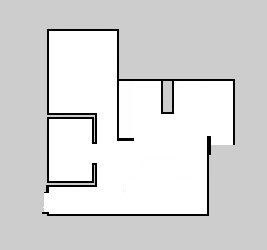
\includegraphics[width=7cm]{img/cap4/mapaestatico}
  \end{center}
  \caption{Mapa estático}
  \label{fig:mapaestatico}
\end{figure}

\subsection{Mapa de corto plazo}
El mapa de corto plazo se caracteriza por ser un mapa en el que se representa los objetos que el robot va percibiendo. Este mapa se inicializa con el valor 255, lo que indica una incertidumbre total. En el instante en el que el algoritmo de construcción del mapa comienza a iterar comenzarán a corregirse estos valores iniciales, asignando el valor 0 a las celdas que corresponden con zonas libres e incrementando desde 0 hasta 254 el valor de las celdas que se perciben como ocupadas. \\

{EJEMPLO CODIGO}\\

El algoritmo propuesto destaca por la capacidad de no solo añadir objetos al mapa, si no ademas eliminarlos si los objetos desaparecen del lugar que ocupaban. Para ello se compara cada muestra de datos con el mapa que estamos generando y si en dicha muestra existen celdas libres que en el mapa están ocupadas se decrementa el valor de dicha celda en el mapa. La cuantia del decremento se puede modelar, consiguiendo asi que el robot olvide más lentamente o más rapidamente los objetos que desaparecen del escenario.\\

{EJEMPLO CODIGO}\\
{EJEMPLO GRAFICO}\\

\subsection{Mapa de largo plazo}
El mapa de largo plazo se inicializa con los valores del mapa estático y se caracteriza por incluir los objetos que tienen un valor muy alto en el mapa de corto plazo, por tanto tenemos un mapa con objetos que han perdurado en el mapa a corto plazo durante un largo periodo de tiempo y que podemos considerar que son objetos estáticos del escenario. 
Este mapa tambien es dinámico, por lo que tambien elimina los objetos del mapa si estos desaparecen del escenario. Para ello se compara el mapa de largo plazo con el mapa de corto plazo. Si una celda en el mapa de largo plazo tiene un valor que indica que está ocupada y en el mapa de corto plazo esa misma celda tiene un valor que indica que está libre, siempre y cuando esa celda no pertenezca a una celda de una pared, se decrementa su valor en el mapa de largo plazo. La cuantia de este decremento tambien puede modelarse, regulando asi la memoria que tenemos de los objetos que hemos añadido a este mapa.\\

{EJEMPLO CODIGO}\\
{EJEMPLO GRAFICO}\\

Adicionalmente este mapa se guarda cada cierto tiempo. Esto nos permite tener una memoria de los objetos que hay en el escenario entre ejecuciones del algoritmo.




\section{Construcción del mapa final}
\label{sec:construccionmap}

